\chapter{Results}
This chapter contains the results of the thesis. First, we look at the outcomes of the user test.
The results are encouraging and we take a closer look at some of them.
Then, small applications demonstrate the usage of the Sequence Library. The
examples show that the concepts and implementations presented in this thesis
are useful in different ways. The following section lists features that have not yet been
implemented. Finally, we will discuss the results obtained in this thesis. For
this purpose, we will take a closer look at the specific topics of this work.
Each topic briefly mentions what was achieved and where there were limits to
it.
\section{User Test Evaluation} % (fold)
\label{sec:User Test Evaluation}
\subsection{Introduction} % (fold)
\label{sub:Introduction}
We conducted user tests with various developers to get feedback on the library.
In total, 13 people participated in this test. All those received a link to a
GitHub repository containing the description of two tasks:
\begin{enumerate}
\item \textbf{Numerical differentiation}: The idea is to use sequences to get
  an approximation as close as possible to the slope of a function |f| at point
  |x|. Lazyness and operations on sequences make this possible.
\item \textbf{Browse JSON files}: In JavaScript you frequently work with JSON
  files provided by some API. This data is often full of holes, which makes it
  difficult to process. JINQ simplifies this task significantly because it
  fills such gaps automatically. 
\end{enumerate}
Both tasks are pleasent use cases of the artifacts of this work.
Chapter~\ref{sec:Examples} describes them in detail.\\
Finally, each participant filled out a questionnaire. This procedure enables
the detection of difficulties and shows where the API still has room for
improvement. 

The findings are based on the questionnaire evaluation and the code of three
participants who handed in their solution. This chapter lists all the
improvements the user test pointed out. In addition, it concludes the general
impression collected by the user test.
Appendix~\ref{chap:app_user_test_results} contains all the user test questions
and their answers.
% subsection Introduction (end)
\subsection{Findings for the Sequence library} % (fold)
\label{sub:Findings for the sequence library}
\subsubsection{General findings and improvements} % (fold)
\label{subsub:Numerical Differentiation Sequence library}
We decided to include following findings in the Sequence library:
\begin{itemize}
  \item \textbf{Renaming untilFunction}: Creating sequences using the sequence
    constructor worked well for everyone. The meaning of the parameters was
    clear to all. (\ref{sub:ut_q3}) However, a suggestion for a meaningful
    optimization from two participants was to rename the |untilFunction| to
    |whileFunction|. This name states clearer that the function should return
    |false| when the sequence ends. (This suggestion was handed in by a
    solution)
  \item \textbf{Better type documentation in JSDoc}: The IDEs have problems
    correctly displaying type information for curried functions (Ref. 2).
    Therefore, the already often used JSDoc annotation "@haskell" , which
    describes the type signature of a function as in Haskell, is added
    everywhere.
\end{itemize}
The following are great ideas but are beyond the scope of this project to
implement. Find detailed information about all of them in the Section~\ref{futu}
\begin{itemize}
  \item \textbf{unfoldr}: The Future Features section explains this
    function. (This suggestion was handed in by a solution)
  \item \textbf{uncons with empty Lists}: as for now, |uncons| is not able to
    handle empty sequences.
\end{itemize}
\subsubsection{Conclusion} % (fold)
\label{subsub:Conclusion}

Almost everyone uses operators as |map|, |filter|, |take|, |reduce|
frequently when working with lists. So the Sequence library brings much-needed
functions. (\ref{sub:ut_q2}) \\ 

Figure~\ref{fig:usertest_q1} concludes the overall opinion about the Sequence
library very well. It shows that most users think that it can be an
advantage in their next project.
\begin{figure}
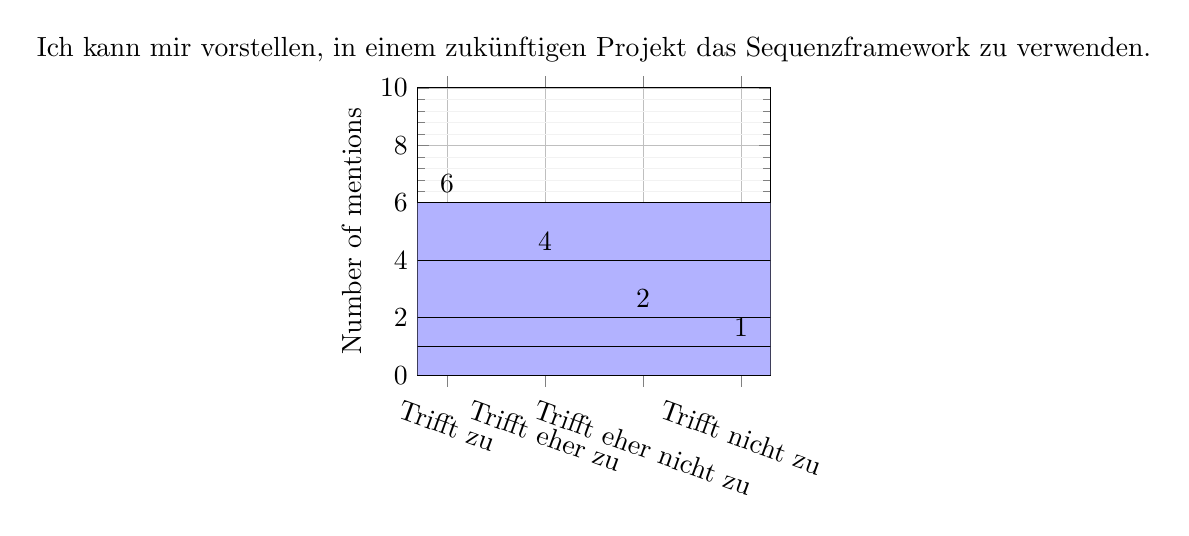
\begin{tikzpicture}
\begin{axis}[
% instead of scaling
width=\textwidth / 2, % Breite des Charts
title={Ich kann mir vorstellen, in einem zukünftigen Projekt das Sequenzframework zu verwenden.},
ybar,  % Art des Charts                                            
ymin=0, % y min
ymax=10, % y max
bar width=20, % Breite der Balken (in points)
nodes near coords, % Labels oberhalb der Bars
ylabel={Number of mentions},
grid=both, % Zeilen ds Grids
grid style={line width=.1pt, draw=gray!10},
major grid style={line width=.2pt,draw=gray!50},
minor y tick num=4,
xtick=data,
% use explicit ticklabels instead of symbolc x coords
xticklabels={Trifft zu, Trifft eher zu, Trifft eher nicht zu, Trifft nicht zu},
xticklabel style={ rotate=-20 },
]
\addplot[black,fill=blue!30!white]
coordinates{ (1,6) (2,4) (3,2) (4,1) };
\end{axis}
\end{tikzpicture}
\caption{Responses to "Ich kann mir vorstellen, in einem zukünftigen Projekt
das Sequenzframework zu verwenden."}
\label{fig:usertest_q1}
\end{figure}
% subsubsection Conclusion (end)
% subsection Findings Sequence library(end)
% section User Test Evaluation (end)

\section{Examples} % (fold)
\label{sec:Examples}

% section Examples (end)

\section{Future Features}
\label{sec:Future Features}
During the project, some ideas emerged that were not feasible for the time
being for various reasons. This section describes these possible extensions for
the standard library.

\subsection{Logging}
\label{sub:Logging}
Logging is a topic that has come up several times. On the one hand, it appears
during the implementation of the Sequence library, but also through feedback
from a test proband of the user test. In the predecessor project, we implemented
a logging framework~\cite{wild_ip5_2023}. This would also be useful to include
in the Sequence library. Especially in case of errors, analyzing debug or
tracing messages from the involved functions would be helpful. Currently, the
logging framework is only included in a part of the test framework. But this
could be extended in a further step.

\subsection{Operators and Operations}
\label{sub:Operators and Operations}
Following are some possible extensions for the Sequence library:

\subsubsection{uncons for empty Sequences}
\label{subsub:uncons}
|uncons| is an operation that returns the head and the rest of an iterable in a
pair. The Sequence library already includes this operation.
But it does not work on empty sequences. Meaning |uncons| applied to an
empty iterable fails. Thus, one would have a version, which for example, wraps the
result in a maybe. |uncons| on an empty list would then return |Nothing|.
The API documentation page~\cite{hoogle_uncons} describes the function in
detail.

\subsubsection{tail}
\label{subsub:tail}
|tail|~\cite{hoogle_tail} is a useful function that removes the first element
of an iterable and returns the rest of it. By implementing |tail|, one has to
pay attention to empty or single-valued iterables, which do not have a tail. An
option could be to return a maybe. |Nothing|, if the list has one or zero
elements, and |Just| including the result otherwise.

\subsubsection{unfoldr}
\label{subsub:unfoldr}
|unfoldr| is a powerful concept for creating lists in Haskell. It would
supplement the options to create new sequences besides the constructor |Sequence|. 
In Haskell, it works using a |Maybe|. |unfoldr| creates a list that returns a
pair wrapped in |Just| with the value of the current iteration and the next
element. If the stop condition is fulfilled, |unfoldr| returns |Nothing|. For
further information, look at the documentation on ~\cite{hoogle_unfoldr}.

\subsubsection{iterate}
\label{subsub:iterate}
|iterate| takes two arguments. The first argument is a function, and the second
is a start value. It generates an infinite iterable of repeated applications of
the function to the calculated value. You will find more information about
|iterate| on hoogle~\cite{hoogle_iterate}.

\subsection{JINQ Functions}
\label{sub:JINQ Functions}
It is possible to get errors when working with |JINQ| and |JSONMonad| by grabbing
not present properties. That means if a function in |select| accesses a property
which is not defined, it will throw an error. This kind of null-case handling
takes a lot of work. To remedy this situation, having error-safe functions like
|safeSelect| to access probably not existing values would be excellent.

\subsection{Applications}
\label{sub:Applications}
\subsubsection{Fix Point Sequence}
\label{subsub:Fixpoint Sequence}
In the mathematical context, having a tool for approximations is helpful. A
constructor for such a case could be the fix point sequence. It allows us to
find an approximation with a given number of iterations or by providing a value
of minimal deviation. The function |within| described in 
section~\ref{sub:Numerical Differentiation} already serves as a good starting
point.

\subsubsection{Use JINQ to process HTML}
\label{subsub:Use JINQ to process HTML}
Scalpel~\cite{scalpel} is a Haskell library to scrap web content. Building a
similar application based on the present implementations could be possible.
With |JINQ| and |JsonMonad|, the standard library already contains a scraping
tool for JSON Objects. A future implementation could use a similar approach to
develop such an application.

\section{Conclusion}
\label{sec:conclusion}
\subsection{Findings and Achievements}
\label{sub:Findings and Achievements}
This thesis aimed to develop a functional standard library for the Kolibri Web
Ui Toolkit in JavaScript. To achieve this, we delved into the iterable
protocols of JavaScript, leveraging our understanding to construct the concept
of sequences. The characteristics of Sequences are lazy evaluation and
immutability, offering a powerful tool for handling any iterable object. By
decorating sequences, a whole library capable of processing, transforming, and
creating sequences arose. This library can also process every iterable object,
such as JavaScript arrays! This was made possible by passing the receiver to
the function, allowing to take advantage of eta reduction.\\
The power of eta reduction manifests itself in the pipe function, enabling the
execution of multiple operations sequentially, dramatically improving code
readability. With the Sequence library’s compatibility with all iterable
objects, it became logical to make other existing collections iterable as well.
As a result, existing Kolibri Toolkit collections, such as pair, stack, and
tuple, are now iterable and, therefore, compatible with the Sequence library!
Many examples show how to build new sequences using the sequence library!\\
Typing the Sequence library using JSDoc ensures clarity and maintains
consistency. Despite some challenges, a powerful functional
standard library for the Kolibri Web Ui Toolkit emerged, offering enhanced
functionality and versatility to JavaScript developers.
\subsection{A Closer Look to Particular Findings}
\label{sub:A Closer Look to Particular Findings}

\subsubsection{Similarity to Haskell}
\label{subsub:Similarity to Haskell}
As Haskell is a well-established and widely used functional language, it serves
as a great role model for solutions to problems when making decisions. \\
However, it is essential to note that some remarkable language concepts of
Haskell do not exist in JavaScript, making it harder to translate code directly
from one language to the other. \\
Nevertheless, specific implementations are
pretty similar, as the following listings~\ref{lst:comparing_with_javascript}
and~\ref{lst:comparing_with_haskell} demonstrate:

\begin{lstlisting}[
  style=Haskell, 
  caption=Haskell vs. Sequence library - Haskell implementation, 
  label={lst:comparing_with_javascript}
  ]
-- Creating a list from 0 to 4
let list = unfoldr (\x -> if x < 5 then Just(x, x + 1) else Nothing) 0

-- mapping the list
map (\x -> x * 2) list 
\end{lstlisting}

\begin{lstlisting}[
  style=ES6, 
  caption=Haskell vs. Sequence library - JavaScript implementation,
  label={lst:comparing_with_haskell}
  ]
// Creating a list from 0 to 4
const list = Sequence(0, x => x < 5, x => x + 1);

// mapping the list
map(x => x * 2)(list)
\end{lstlisting}
\subsubsection{Robust Programming in JavaScript}
\label{subsub:Robust Programming in JavaScript}
Strange situations arise in JavaScript more often than in other programming
languages. One contributing factor is the nature of its type system. However,
this thesis demonstrates that functional programming concepts and distinct
usage of JSDoc allow the development of reasonably robust programs.\\
Crucially, this requires taking advantage of the functional aspects inherent to
the language, such as higher-order functions and partial application.
Nevertheless, certain limitations sometimes pose significant problems on the
solution path. In particular, not all desired behaviors are achievable when
dealing with the type system: JSDoc is very limited when combining multiple
types or writing general functions that need types to abstract over another
type. An illustrative example of this is the combination of a MonadType with an
Iterable type: When a function returns a MonadType, the valuable information
that this monad could also be iterable is lost. Resolving such a situation
requires type-casting.
\subsubsection{Monadic Structures}
\label{subsub:Monadic Structures}
|JINQ| explained in section ~\ref{sec:Query different Data Structures}, is a
concept based on monadic types. This shows that implementing such concepts in
JavaScript is also possible and valuable, which opens numerous possibilities
for extensions that act on monadic types in JavaScript.

\subsubsection{Testing}
\label{subsub:Testing}
A reliable test framework is crucial for achieving a robust and sustainable
library. In the case of the Sequence library, the testing table attained the
stability of the Sequence library. This lies a solid foundation for incremental
growth. The library's core became increasingly robust by gradually
incorporating new functionalities and corresponding test cases. Moreover, novel
test concepts were introduced during the development process to enhance the
testing capabilities further. A notable example is the introduction of
invariant tests (section~\ref{sub:Invariant Testing}), which systematically
assess the behaviours of functionalities through diverse testing approaches,
ensuring comprehensive validation.

\subsection{Non-Functional Findings}
\label{sub:Non-Functional Aspects}
\subsubsection{Library Organization}
\label{subsub:Library Organisation}
During the development of the Sequence library, we consistently paid close
attention to non-functional aspects. As part of this effort, we adjusted the
organization of the project's development setup. This led to the current state,
where each operation of the Sequence library is in a separate file. Adopting
such a project structure has significantly impacted the codebase's overall
clarity and navigability. Moreover, it contributes to a sense of order, which,
in turn, enhances the overall code quality. Additionally, it helps to prevent
cycling dependencies when importing particular functionalities.
\subsubsection{Code Quality}
\label{subsub:Code Quality}
Maintaining high code quality standards led to a clear and consistent
code base. Several points were particularly important during development:
\begin{itemize}
  \item{No code duplications}
  \item{Good naming}
  \item{Standardized formatting}
  \item{Only necessary exports of functions}
  \item{Appropriate comments and JSDoc}
  \item{Project organization and structure}
\end{itemize}

Strict adherence to these principles made development easier for us and helps
library users find their way around more quickly. Additionally, it facilitates
future developers to learn how to add new functionalities.

\subsection{User Testing}
\label{sub:User Testing}
The user testing conducted in section~\ref{sub:User Testing} was crucial for
assessing the usefulness of the Sequence library. It provided valuable feedback
from programmers without prior knowledge of the library. These insights allowed
for addressing specific issues and offered helpful improvements. Additionally,
other useful suggestions contributed to the list of potential enhancements, as
outlined in section ~\ref{sec:Future Features}.

